\section{Kiến thức nền tảng}

Chương này trình bày các kiến thức trực tiếp phục vụ việc xây dựng trợ lý mua sắm đa phương thức. Hệ thống kết hợp xử lý ngôn ngữ tự nhiên, truy hồi sản phẩm bằng vector, tìm kiếm bằng hình ảnh và Retrieval-Augmented Generation (RAG) để hỗ trợ tìm kiếm bằng văn bản, bằng ảnh và kết hợp văn bản--ảnh. Các công nghệ, thư viện và mô hình cụ thể được trình bày ở chương tiếp theo; chương này tập trung vào nguyên lý hoạt động.

\subsection{Bài toán trợ lý mua sắm đa phương thức}

\subsubsection{Tìm kiếm sản phẩm bằng ngôn ngữ tự nhiên}

Trong thương mại điện tử, tìm kiếm sản phẩm là quá trình ánh xạ nhu cầu của người dùng tới các sản phẩm phù hợp trong danh mục. Ngoài tên và mô tả, mỗi sản phẩm còn có các thuộc tính như danh mục, thương hiệu, màu sắc, chất liệu, kích thước, đối tượng sử dụng, giá bán và trạng thái kinh doanh. Vì vậy, mức độ phù hợp không chỉ phụ thuộc vào việc truy vấn và tên sản phẩm có chung từ khóa hay không, mà còn phụ thuộc vào việc sản phẩm có thỏa mãn các điều kiện cụ thể của người dùng hay không.

Người dùng thường diễn đạt nhu cầu dưới dạng câu tự nhiên, chẳng hạn “tìm váy dự tiệc màu đỏ, cổ tim, giá dưới 1 triệu”. Truy vấn này chứa đồng thời loại sản phẩm, mục đích sử dụng, màu sắc, kiểu dáng và giới hạn giá. Hệ thống phải nhận diện ý định, trích xuất thuộc tính, phân biệt điều kiện bắt buộc với sở thích mềm, sau đó truy hồi và xếp hạng sản phẩm. Trong hội thoại nhiều lượt, truy vấn hiện tại còn có thể phụ thuộc vào ngữ cảnh trước đó, ví dụ “có mẫu tương tự nhưng rẻ hơn không?”.

\subsubsection{Hạn chế của tìm kiếm dựa trên từ khóa}

Tìm kiếm dựa trên từ khóa đối sánh trực tiếp các token của truy vấn với tên hoặc mô tả sản phẩm. Cách tiếp cận này nhanh, dễ giải thích và hiệu quả đối với tên sản phẩm, thương hiệu hoặc cụm từ chính xác. Tuy nhiên, phương pháp này không tự biểu diễn được quan hệ ngữ nghĩa giữa các cách diễn đạt khác nhau. Một sản phẩm có tên “sneaker nữ phong cách thể thao” vẫn có thể phù hợp với truy vấn “giày nữ đi học” dù hai chuỗi không trùng khớp hoàn toàn.

Các hạn chế thường gặp gồm từ đồng nghĩa, truy vấn không dấu, lỗi chính tả, cách gọi tiếng Việt và tiếng Anh xen kẽ, truy vấn dài và yêu cầu mô tả phong cách. Do đó, đồ án không xem đối sánh từ khóa là cơ chế truy hồi duy nhất. Tín hiệu từ khóa chính xác được giữ lại để hỗ trợ truy vấn tên sản phẩm, trong khi tìm kiếm ngữ nghĩa và lọc metadata xử lý ý định cùng các ràng buộc phức tạp hơn.

\subsubsection{Tìm kiếm ngữ nghĩa và tìm kiếm đa phương thức}

Tìm kiếm ngữ nghĩa biểu diễn truy vấn và sản phẩm dưới dạng vector trong không gian nhiều chiều. Các đối tượng có nội dung gần nhau được kỳ vọng có vector gần nhau, nhờ đó hệ thống có thể truy hồi sản phẩm phù hợp dù từ ngữ không trùng khớp hoàn toàn. Quy trình cơ bản gồm xử lý truy vấn, sinh embedding, tìm kiếm vector và xếp hạng kết quả.

\begin{figure}[H]
    \centering
    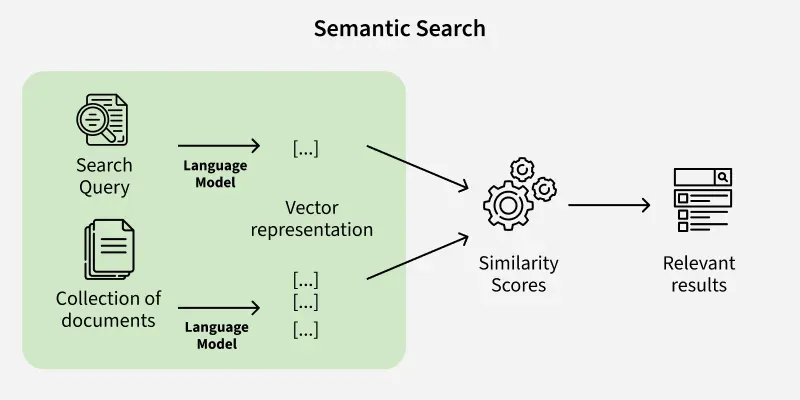
\includegraphics[width=0.75\textwidth]{Images/Kienthucnentang/Semantic-Search.png}
    \caption{Quy trình tìm kiếm ngữ nghĩa từ truy vấn đến kết quả xếp hạng \parencite{geeksforgeeks_semantic_search}}
    \label{fig:semantic_search_pipeline}
\end{figure}

Tìm kiếm đa phương thức mở rộng bài toán bằng cách tiếp nhận nhiều dạng dữ liệu. Trong phạm vi đồ án, hai modality chính là văn bản và hình ảnh. Người dùng có thể tải ảnh để tìm sản phẩm tương tự, hoặc kết hợp ảnh với mô tả như “tìm mẫu giống ảnh này nhưng màu đen”. Hệ thống khi đó phải khai thác cả đặc trưng thị giác, ngữ nghĩa văn bản và metadata sản phẩm trước khi tạo thứ hạng cuối cùng.

\begin{figure}[H]
    \centering
    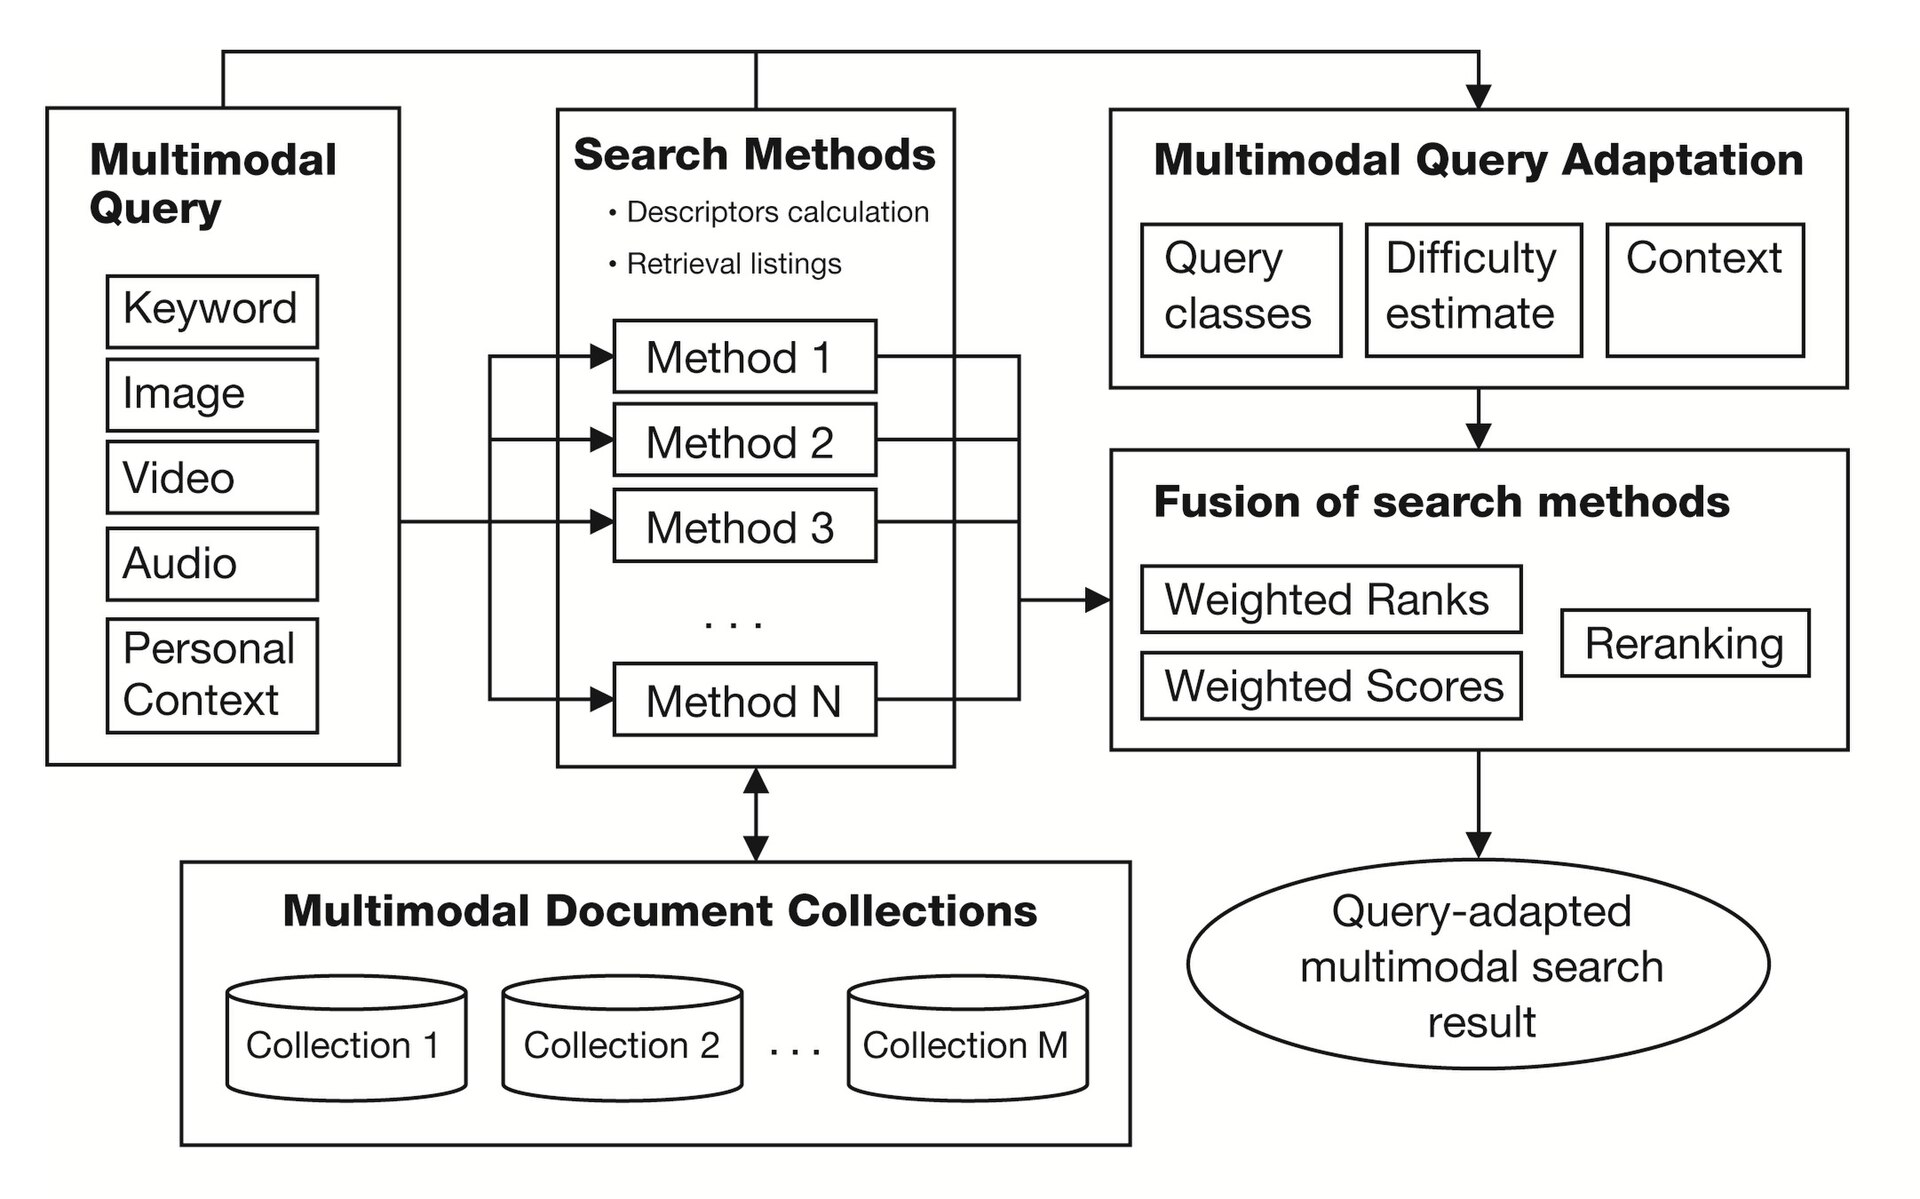
\includegraphics[width=0.72\textwidth]{Images/Kienthucnentang/Framework_of_Multimodal_Search.jpg}
    \caption{Khái quát hệ thống tìm kiếm kết hợp truy vấn văn bản và hình ảnh \parencite{ipullrank_mum_search}}
    \label{fig:multimodal_search_overview}
\end{figure}

\subsection{Biểu diễn embedding đa phương thức}

\subsubsection{Vector embedding và không gian ngữ nghĩa}

Vector embedding là phép ánh xạ một đối tượng như câu văn, hình ảnh hoặc sản phẩm thành vector số thực có số chiều cố định. Embedding được học từ dữ liệu để lưu giữ các đặc trưng có ích cho việc so sánh ngữ nghĩa \parencite{pinecone_embedding}. Tập các vector tạo thành không gian embedding, trong đó vị trí tương đối giữa các vector phản ánh mức độ liên quan theo cách mà mô hình đã học.

Trong đồ án, dữ liệu sản phẩm được embedding trước và lưu vào cơ sở dữ liệu vector. Khi tìm kiếm, truy vấn mới được đưa qua mô hình tương ứng để sinh vector, sau đó so sánh với các vector đã lập chỉ mục. Chất lượng embedding ảnh hưởng trực tiếp đến khả năng nhận biết từ đồng nghĩa, phong cách, loại sản phẩm và sự tương đồng thị giác.

\subsubsection{Embedding văn bản}

Text embedding chuyển câu truy vấn hoặc nội dung sản phẩm thành vector ngữ nghĩa. Nội dung biểu diễn sản phẩm có thể tổng hợp từ tên, mô tả, danh mục và các thuộc tính liên quan. Semantic retrieval sau đó tìm các sản phẩm có vector gần với vector truy vấn.

Embedding giúp giảm sự phụ thuộc vào đối sánh bề mặt. Chẳng hạn, “váy đi tiệc” và “đầm dự sự kiện” có thể được xem là gần nhau về nhu cầu sử dụng. Tuy vậy, embedding không thay thế hoàn toàn việc trích xuất điều kiện. Các ràng buộc chính xác như mức giá tối đa hoặc trạng thái còn bán cần được xử lý bằng metadata filtering.

\subsubsection{Embedding hình ảnh}

Image embedding chuyển hình ảnh thành vector đặc trưng biểu diễn các yếu tố thị giác như hình dạng, màu sắc, họa tiết, chất liệu biểu kiến và kiểu dáng. Khi người dùng tải ảnh, hệ thống sinh vector cho ảnh truy vấn rồi thực hiện tìm kiếm tương đồng trên các vector ảnh sản phẩm. Đây là nền tảng của image-to-product retrieval và visual search.

Ảnh đầu vào cần được chuẩn hóa về định dạng, kích thước và hướng ảnh trước khi sinh embedding. Nếu ảnh chứa nhiều vật thể hoặc phần nền lớn, một vùng quan tâm có thể được người dùng chọn hoặc được bộ phát hiện đối tượng đề xuất. Ảnh toàn phần vẫn là đầu vào dự phòng để tránh làm mất sản phẩm khi bước phát hiện không chắc chắn.

\subsubsection{Không gian embedding chung cho văn bản và hình ảnh}

Multimodal embedding ánh xạ văn bản và hình ảnh vào một không gian tương thích. Các mô hình thị giác--ngôn ngữ thường sử dụng hai encoder cho hai modality và huấn luyện theo mục tiêu tương phản để đưa các cặp văn bản--ảnh phù hợp lại gần nhau \parencite{clip_paper}. Nhờ đó, hệ thống có thể thực hiện text-to-image, image-to-image và truy hồi kết hợp.

\begin{figure}[H]
    \centering
    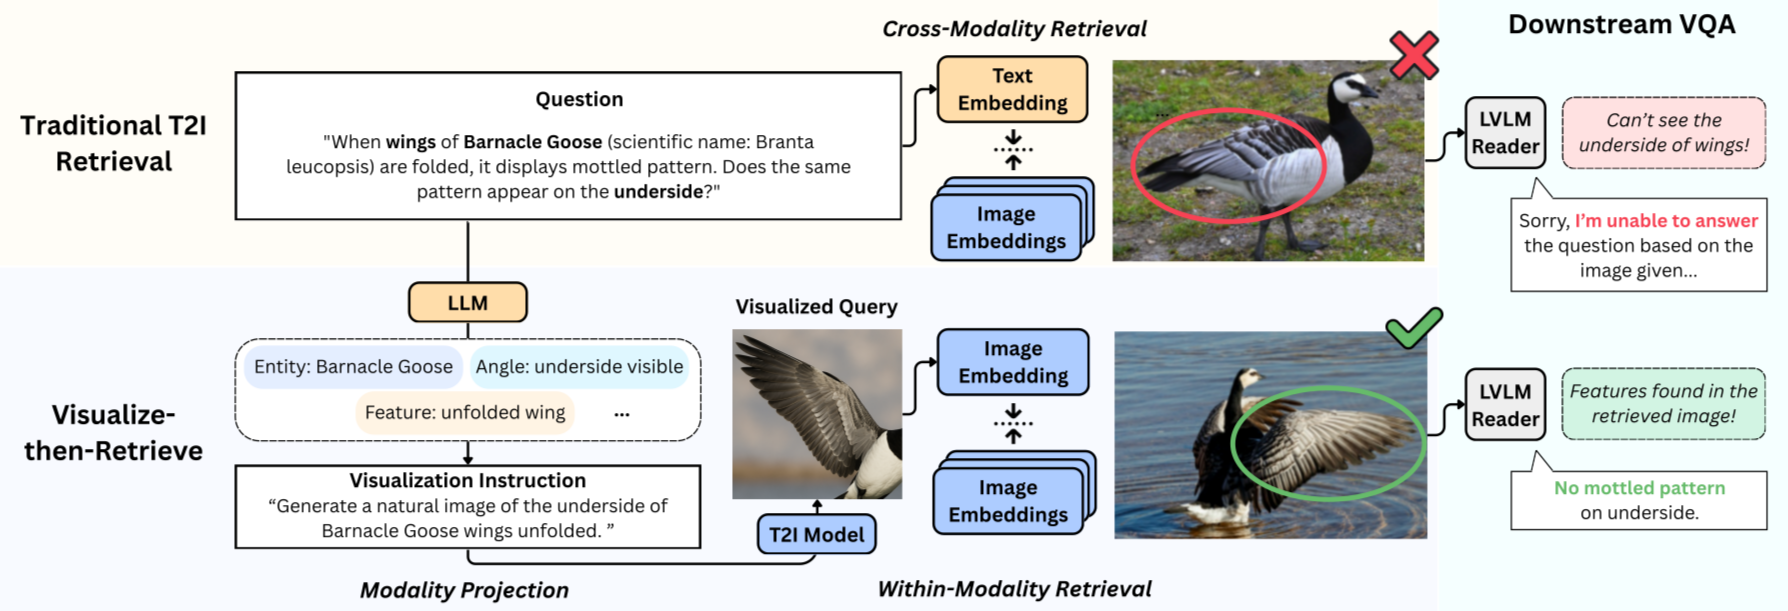
\includegraphics[width=0.78\textwidth]{Images/Kienthucnentang/text-image-retrieval.png}
    \caption{Ánh xạ văn bản và hình ảnh vào không gian biểu diễn chung để thực hiện truy hồi đa phương thức \parencite{faghri2018vsepp}}
    \label{fig:text_image_retrieval}
\end{figure}

Trong đồ án, văn bản và hình ảnh tạo thành hai nhánh truy hồi. Kết quả của mỗi nhánh được hợp nhất theo sản phẩm, sau đó kết hợp với mức khớp thuộc tính và tín hiệu nghiệp vụ. Cách tổ chức này cho phép hệ thống tận dụng không gian embedding chung nhưng vẫn kiểm soát riêng đóng góp của từng modality.

\subsection{Truy hồi vector}

\subsubsection{Cơ sở dữ liệu vector}

Cơ sở dữ liệu vector quản lý embedding cùng metadata và cung cấp phép tìm kiếm các vector gần nhất \parencite{wang2021milvus}. Mỗi điểm dữ liệu thường gồm định danh, vector và payload mô tả đối tượng. Trong bài toán sản phẩm, payload có thể chứa mã sản phẩm, danh mục, thương hiệu, màu, chất liệu, kích thước, giới tính, giá bán và trạng thái hoạt động.

Việc lưu vector cùng payload cho phép hệ thống kết hợp similarity search với điều kiện lọc. Ví dụ, sau khi biểu diễn ngữ nghĩa của “váy dự tiệc”, truy vấn vector có thể đồng thời giới hạn màu đỏ, giá không vượt quá một triệu đồng và chỉ lấy sản phẩm đang hoạt động.

\subsubsection{Độ tương đồng vector}

Độ tương đồng vector định lượng mức độ gần nhau giữa vector truy vấn và vector sản phẩm. Các phép đo phổ biến gồm cosine similarity, dot product và Euclidean distance. Cosine similarity đo góc giữa hai vector và thường được sử dụng khi hướng của vector quan trọng hơn độ lớn \parencite{qdrant2024vectorsimilarity}:

\begin{equation}
    \operatorname{cos}(\mathbf{q},\mathbf{x})=
    \frac{\mathbf{q}\cdot\mathbf{x}}
    {\lVert\mathbf{q}\rVert_2\lVert\mathbf{x}\rVert_2}.
    \label{eq:cosine_similarity}
\end{equation}

Trong đó, $\mathbf{q}$ là vector truy vấn và $\mathbf{x}$ là vector sản phẩm. Điểm tương đồng là tín hiệu quan trọng cho xếp hạng nhưng không phải tín hiệu duy nhất; hệ thống còn phải xét điều kiện lọc, mức khớp thuộc tính và các tín hiệu nghiệp vụ.

\begin{figure}[H]
    \centering
    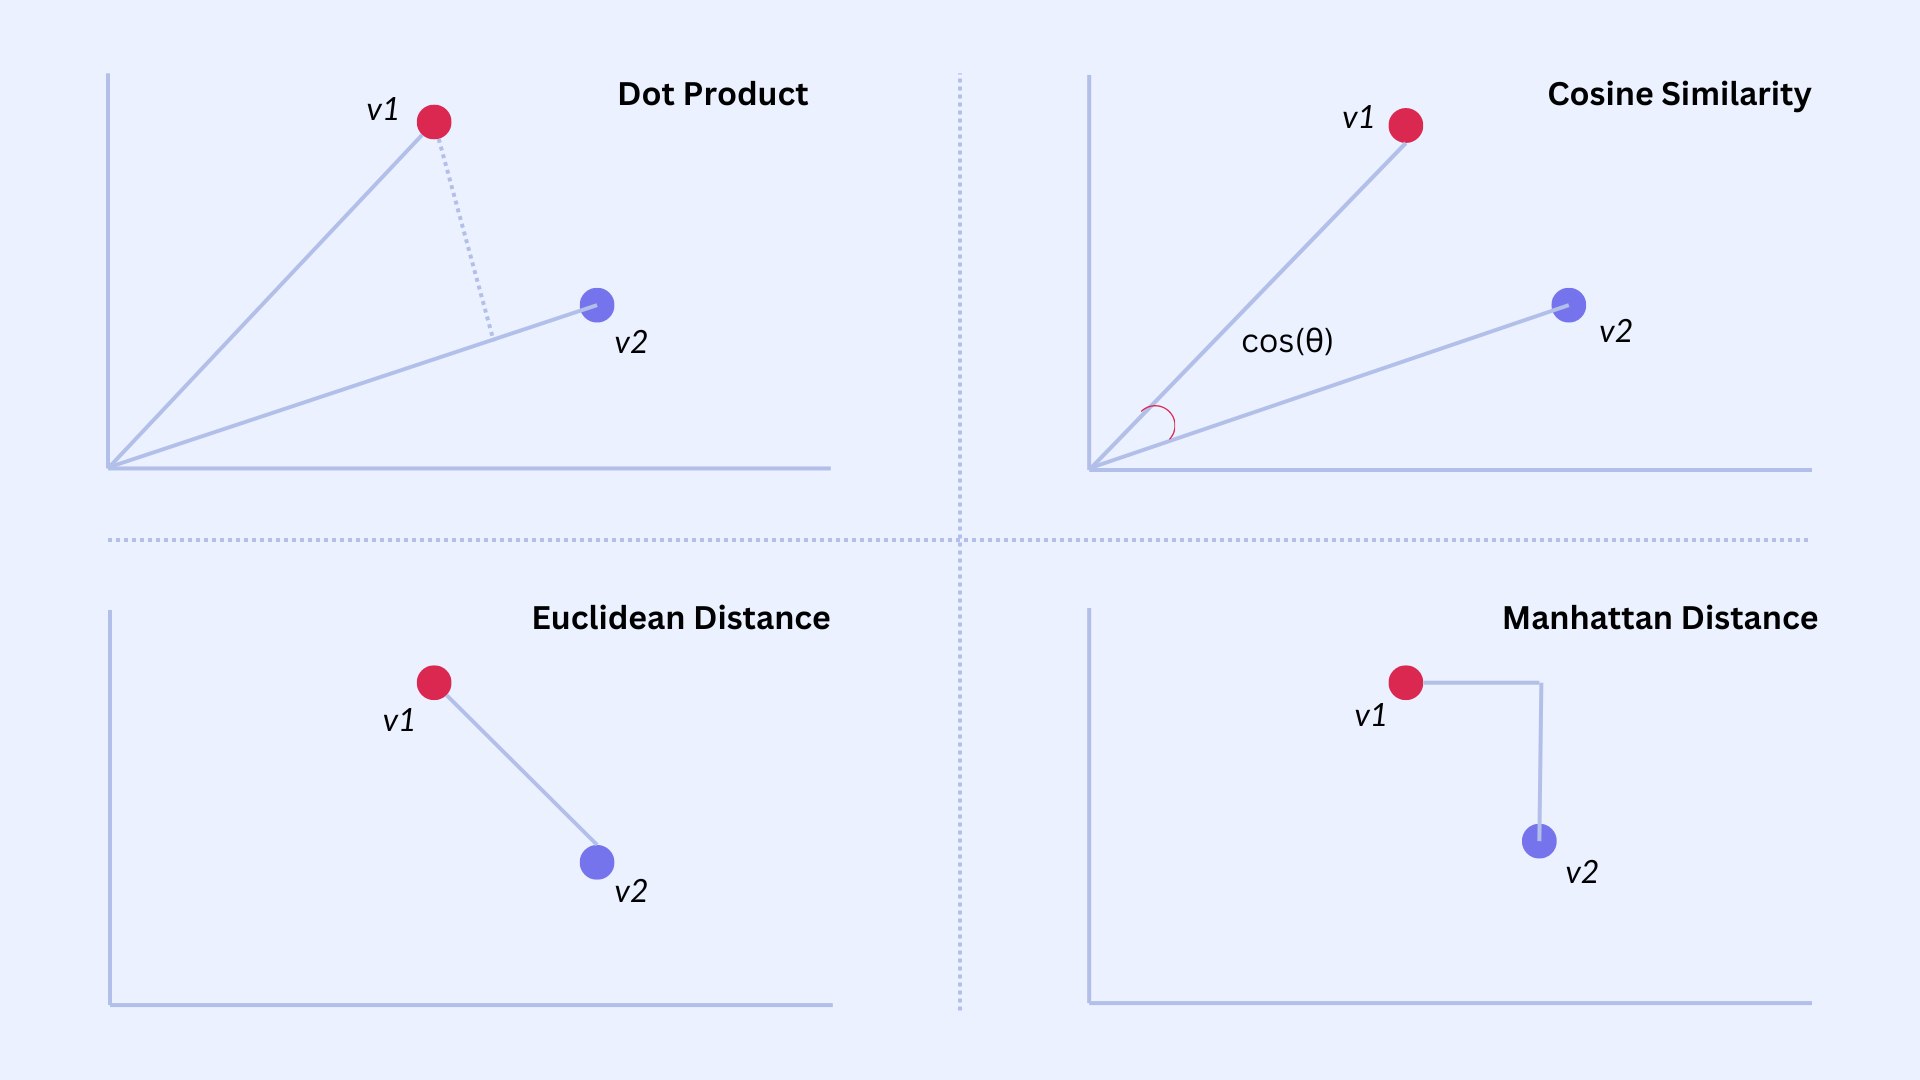
\includegraphics[width=0.72\linewidth]{Images/Kienthucnentang/vector-similarity.png}
    \caption{Các vector có nội dung tương tự được phân bố gần nhau trong không gian embedding \parencite{qdrant2024vectorsimilarity}}
    \label{fig:vector_similarity}
\end{figure}

\subsubsection{Approximate Nearest Neighbor và HNSW}

Với số lượng vector lớn, so sánh truy vấn với mọi vector có chi phí tuyến tính theo kích thước dữ liệu. Approximate Nearest Neighbor (ANN) giảm chi phí bằng cách tìm tập lân cận gần đúng thay vì bảo đảm duyệt toàn bộ không gian \parencite{arya1998optimal}. Sự đánh đổi này phù hợp với hệ thống tìm kiếm tương tác vì giảm độ trễ trong khi vẫn duy trì chất lượng truy hồi ở mức cao.

Hierarchical Navigable Small World (HNSW) là một phương pháp ANN dựa trên đồ thị nhiều tầng \parencite{malkov2018efficient}. Các tầng trên chứa liên kết thưa để di chuyển nhanh giữa các vùng xa, còn tầng thấp chứa liên kết dày hơn để tinh chỉnh lân cận.

\begin{figure}[H]
    \centering
    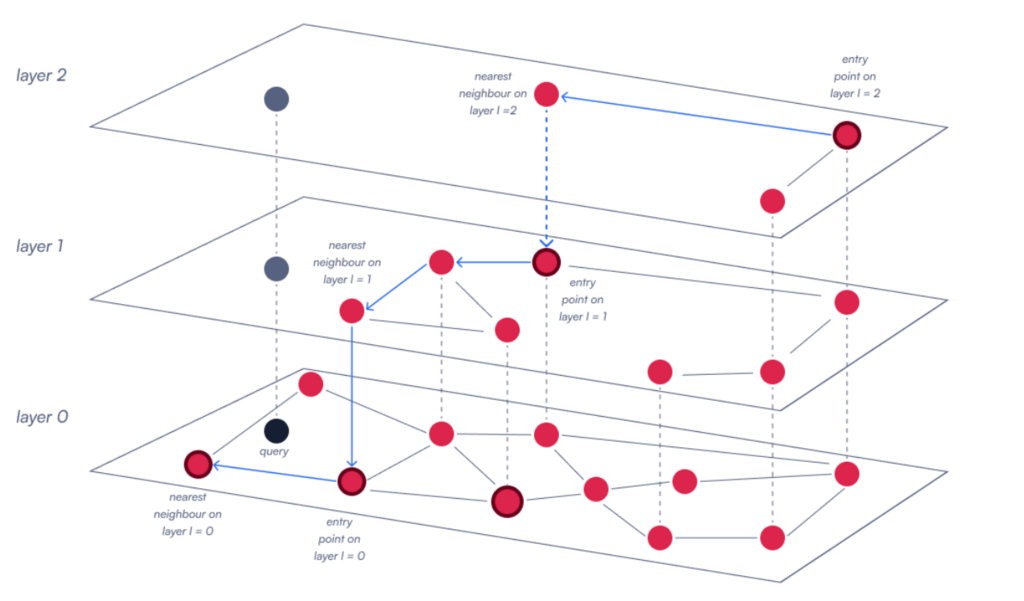
\includegraphics[width=0.72\linewidth]{Images/Kienthucnentang/hnsw-overview.png}
    \caption{Cấu trúc đồ thị nhiều tầng của HNSW trong tìm kiếm lân cận gần đúng \parencite{qdrant2024hnsw}}
    \label{fig:hnsw_overview}
\end{figure}

\subsection{Hiểu và xử lý truy vấn sản phẩm}

\subsubsection{Phân tích ý định và trích xuất thuộc tính}

Query understanding là quá trình xác định mục đích và các thông tin có cấu trúc trong phát biểu của người dùng \parencite{guo2020deep}. Đối với trợ lý mua sắm, các ý định quan trọng gồm tìm kiếm bằng văn bản, tìm kiếm bằng ảnh, tìm kiếm kết hợp, hỏi thông tin sản phẩm, so sánh, làm rõ yêu cầu và tiếp tục hội thoại.

Sau khi nhận diện ý định, hệ thống trích xuất các thuộc tính như danh mục, thương hiệu, màu sắc, chất liệu, kích thước, giới tính, mục đích sử dụng và khoảng giá. Kết quả phân tích có cấu trúc để các bước phía sau có thể kiểm tra, chuẩn hóa và áp dụng nhất quán. Cách tiếp cận kết hợp luật xác định với LLM giúp xử lý nhanh các mẫu rõ ràng, đồng thời hỗ trợ truy vấn tự nhiên và phụ thuộc ngữ cảnh.

\subsubsection{Chuẩn hóa, ánh xạ bí danh và viết lại truy vấn}

Ngôn ngữ tìm kiếm sản phẩm có nhiều biến thể: có dấu hoặc không dấu, tên tiếng Việt hoặc tiếng Anh, cách viết tắt, lỗi gõ và tên gọi không thống nhất. Chuẩn hóa truy vấn đưa các biểu diễn này về dạng nhất quán; ánh xạ bí danh liên kết các cách gọi tương đương với danh mục và thuộc tính chuẩn của hệ thống.

Query rewrite tạo một biểu diễn phù hợp hơn cho bước embedding và retrieval nhưng phải bảo toàn ý định ban đầu \parencite{ren2010query}. Với hội thoại nhiều lượt, truy vấn viết lại có thể bổ sung ngữ cảnh còn hiệu lực. Sau yêu cầu “tìm váy dự tiệc màu đỏ”, câu “loại dưới 800 nghìn” có thể được diễn giải thành truy vấn đầy đủ chứa cả loại sản phẩm, mục đích, màu sắc và giới hạn giá mới.

Việc viết lại không được tự tạo thêm ràng buộc mà người dùng chưa yêu cầu. Giá trị do câu chữ hiện tại nêu rõ có độ tin cậy cao hơn thuộc tính chỉ được suy ra từ mô hình. Nguyên tắc này giúp hạn chế việc loại bỏ sản phẩm phù hợp do diễn giải quá mức.

\subsubsection{Ràng buộc cứng, ràng buộc mềm và metadata filtering}

Metadata filtering áp dụng điều kiện có cấu trúc lên tập ứng viên. Một số điều kiện mang tính bắt buộc, chẳng hạn giá tối đa, thương hiệu được nêu trực tiếp hoặc trạng thái sản phẩm đang bán. Những điều kiện này được xem là ràng buộc cứng và có thể dùng để loại sản phẩm không thỏa mãn.

Ngược lại, thuộc tính chỉ được suy ra hoặc có tính chủ quan như phong cách, dịp sử dụng và một số sắc độ màu nên được xem là ràng buộc mềm. Thay vì loại bỏ ứng viên, hệ thống có thể cộng điểm cho sản phẩm phù hợp. Khi ràng buộc suy diễn làm tập kết quả quá hẹp, cơ chế recovery có thể nới điều kiện mềm nhưng vẫn giữ nguyên các yêu cầu rõ ràng của người dùng.

Việc phân biệt nguồn gốc ràng buộc giúp cân bằng precision và recall. Hard filter cải thiện tính tuân thủ đối với yêu cầu chính xác, còn soft boost giảm nguy cơ bỏ sót do metadata chưa đầy đủ hoặc mô hình hiểu truy vấn chưa chắc chắn.

\subsection{Tìm kiếm đa phương thức và xếp hạng}

\subsubsection{Truy hồi bằng văn bản và hình ảnh}

Nhánh văn bản sinh embedding cho truy vấn đã được chuẩn hóa, truy hồi trên tập vector văn bản và kết hợp các kết quả khớp tên chính xác. Nhánh hình ảnh chuẩn hóa ảnh đầu vào, sinh image embedding và truy hồi trên tập vector ảnh. Do một sản phẩm có thể có nhiều ảnh, kết quả ảnh cần được quy về mức sản phẩm và loại bỏ định danh trùng lặp trước khi trả về.

Đối với ảnh có nhiều đối tượng, Object Detection có thể hỗ trợ xác định bounding box và crop vùng chứa sản phẩm \parencite{redmon2016yolo}. Kết quả phát hiện thường gồm nhãn, tọa độ và confidence score. Trong phạm vi đồ án, đây là bước tăng cường tùy chọn; ảnh toàn phần vẫn được sử dụng khi bộ phát hiện bị tắt hoặc không tìm được vùng đủ tin cậy.

\subsubsection{Hybrid multimodal retrieval}

Khi truy vấn đồng thời có văn bản và hình ảnh, hai nhánh retrieval có thể chạy độc lập rồi hợp nhất theo mã sản phẩm. Một sản phẩm có thể xuất hiện ở một hoặc cả hai nhánh. Cách tiếp cận này giữ được thông tin riêng của từng modality và cho phép quan sát đóng góp của văn bản so với hình ảnh.

Ví dụ, với ảnh một chiếc váy và yêu cầu “mẫu tương tự nhưng màu đen, dưới một triệu”, nhánh ảnh tập trung vào kiểu dáng và đặc trưng thị giác; nhánh văn bản biểu diễn phần mô tả; metadata filtering kiểm soát màu và giá. Kết quả cuối cần thỏa mãn ràng buộc rõ ràng, đồng thời vẫn gần ảnh tham chiếu.

\subsubsection{Weighted fusion và reranking}

Fusion kết hợp nhiều tín hiệu thành điểm xếp hạng chung. Với sản phẩm $p$, điểm có thể được biểu diễn tổng quát như sau:

\begin{equation}
    S(p)=w_iS_i(p)+w_tS_t(p)+w_fS_f(p)+w_bS_b(p)+S_u(p),
    \label{eq:multimodal_fusion}
\end{equation}

trong đó $S_i$ và $S_t$ lần lượt là độ tương đồng ảnh và văn bản; $S_f$ là mức khớp ràng buộc mềm; $S_b$ là tín hiệu nghiệp vụ; $S_u$ là phần tăng cường theo mục đích sử dụng; các hệ số $w$ kiểm soát đóng góp của từng tín hiệu. Các điểm số cần được đưa về thang đo tương thích trước khi cộng có trọng số.

Sau bước truy hồi ban đầu, reranking đánh giá lại một tập ứng viên nhỏ để cải thiện thứ tự kết quả \parencite{reranking_sbert}. Vì reranking tăng chi phí và độ trễ, nó chỉ nên áp dụng lên top-$k$ ứng viên và được bật khi thử nghiệm chứng minh lợi ích về chất lượng.

\subsection{Large Language Model và Retrieval-Augmented Generation}

\subsubsection{Vai trò của Large Language Model}

Large Language Model (LLM) là mô hình học sâu có khả năng hiểu và sinh ngôn ngữ tự nhiên, thường dựa trên kiến trúc Transformer và cơ chế self-attention \parencite{vaswani2017attention}. Trong trợ lý mua sắm, LLM hỗ trợ phân loại ý định, trích xuất thuộc tính, viết lại truy vấn theo ngữ cảnh và tạo phản hồi hội thoại.

LLM không nên tự suy đoán giá, tồn kho hoặc thuộc tính sản phẩm. Những dữ kiện này thay đổi theo dữ liệu nghiệp vụ và cần được lấy từ các dịch vụ của hệ thống. Vai trò phù hợp của LLM là diễn giải nhu cầu và tổng hợp thông tin đã được truy hồi thành câu trả lời dễ hiểu.

\subsubsection{Prompt và đầu ra có cấu trúc}

Prompt là tập hướng dẫn và ngữ cảnh được cung cấp cho LLM. Một prompt cho trợ lý mua sắm thường gồm vai trò của hệ thống, yêu cầu của người dùng, lịch sử hội thoại liên quan, các ràng buộc an toàn, dữ liệu sản phẩm đã truy hồi và định dạng đầu ra mong muốn.

Ở bước hiểu truy vấn, đầu ra có cấu trúc giúp kiểm tra các trường như intent, rewritten query, category, color và price range trước khi truy hồi. Ở bước sinh câu trả lời, prompt cần yêu cầu mô hình chỉ sử dụng dữ kiện được cung cấp, không khẳng định trạng thái tồn kho hoặc thuộc tính không có trong context. Việc tách prompt phân tích khỏi prompt trả lời làm giảm sự phụ thuộc giữa điều phối nghiệp vụ và cách diễn đạt ngôn ngữ.

\subsubsection{Kiến trúc product-grounded RAG}

Retrieval-Augmented Generation kết hợp một thành phần truy hồi với một mô hình sinh để tạo phản hồi dựa trên dữ liệu bên ngoài \parencite{lewis2020rag}. Trong RAG tổng quát, retriever tìm các tài liệu liên quan và generator sử dụng chúng làm context. Đối với đồ án, đơn vị được truy hồi là sản phẩm thay vì đoạn văn thuần túy, vì vậy có thể xem đây là kiến trúc product-grounded RAG.

\begin{figure}[H]
    \centering
    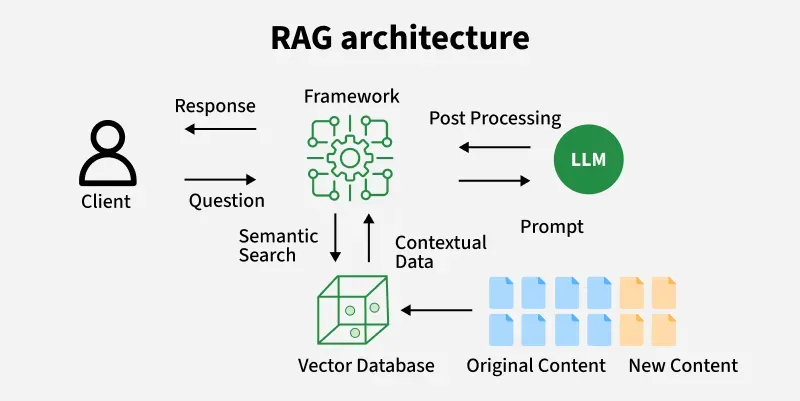
\includegraphics[width=0.75\textwidth]{Images/Kienthucnentang/RAG-architecture.png}
    \caption{Kiến trúc RAG kết hợp truy hồi dữ liệu và sinh phản hồi \parencite{geeksforgeeks2026ragarchitecture}}
    \label{fig:rag_architecture}
\end{figure}

Quy trình product-grounded RAG của trợ lý mua sắm gồm các bước chính:

\begin{enumerate}
    \item Phân tích ý định, truy vấn và các ràng buộc của người dùng.
    \item Truy hồi ứng viên bằng nhánh văn bản, hình ảnh hoặc hybrid.
    \item Lấy metadata và trạng thái kinh doanh hiện hành của các sản phẩm ứng viên.
    \item Xây dựng context có cấu trúc từ các dữ kiện đã xác minh.
    \item Yêu cầu LLM tổng hợp câu trả lời và giải thích gợi ý dựa trên context.
\end{enumerate}

Kiến trúc này giúp giảm hallucination và làm cho phản hồi có căn cứ hơn. Tuy nhiên, RAG không tự bảo đảm tính đúng đắn: chất lượng cuối cùng còn phụ thuộc vào recall của retriever, tính mới của dữ liệu nghiệp vụ, cách xây dựng context và mức độ tuân thủ prompt của generator.

\subsubsection{Bộ nhớ hội thoại}

Conversation memory duy trì thông tin cần thiết giữa các lượt trao đổi. Bộ nhớ có thể chứa tiêu chí đang áp dụng, giá trị đã bị thay thế, sản phẩm người dùng vừa tham chiếu, quyết định đã xác nhận và câu hỏi còn chưa được làm rõ. Nhờ đó, trợ lý có thể xử lý những phát biểu rút gọn như “mẫu thứ hai”, “đổi sang màu đen” hoặc “rẻ hơn một chút”.

Bộ nhớ hội thoại có thể kết hợp lịch sử gần nhất, bản tóm tắt hội thoại và trạng thái có cấu trúc. Lịch sử giữ nguyên cách diễn đạt gần đây; bản tóm tắt giới hạn kích thước context; trạng thái có cấu trúc giúp truy cập chính xác các ràng buộc đang có hiệu lực. Dữ liệu cần được phân tách theo người dùng và phiên hội thoại, đồng thời có chính sách giới hạn dung lượng và thời gian lưu trữ.

\subsection{Đánh giá chất lượng hệ thống}

\subsubsection{Các chỉ số đánh giá truy hồi}

Đánh giá retrieval cần xem xét cả khả năng tìm đúng sản phẩm và chất lượng thứ hạng. Với tập kết quả top-$k$, các chỉ số phù hợp gồm:

\begin{itemize}
    \item \textbf{Hit@$k$}: cho biết ít nhất một sản phẩm liên quan có xuất hiện trong top-$k$ hay không.
    \item \textbf{Precision@$k$}: tỷ lệ sản phẩm liên quan trong $k$ kết quả đầu.
    \item \textbf{Recall@$k$}: tỷ lệ sản phẩm liên quan đã được tìm thấy trong top-$k$ so với toàn bộ tập liên quan.
    \item \textbf{MRR}: trung bình nghịch đảo thứ hạng của kết quả đúng đầu tiên.
    \item \textbf{nDCG@$k$}: đánh giá thứ hạng khi sản phẩm có nhiều mức độ liên quan khác nhau và giảm trọng số ở các vị trí thấp.
\end{itemize}

Các chỉ số cần được diễn giải theo cách xây dựng ground truth. Ví dụ, Recall@$k$ không phản ánh đầy đủ khả năng bao phủ toàn danh mục nếu tập nhãn chỉ được tạo từ chính các ứng viên của một lần chạy. Đối với tìm kiếm ảnh, cần phân biệt truy hồi đúng sản phẩm gốc với truy hồi các sản phẩm tương tự về mặt thị giác.

\subsubsection{Grounding và chất lượng phản hồi}

Đối với RAG, tìm đúng sản phẩm chưa đủ; câu trả lời còn phải sử dụng đúng dữ kiện trong context. Grounding đo mức độ các khẳng định về tên, giá, màu, chất liệu hoặc tình trạng bán được hỗ trợ bởi dữ liệu đã truy hồi. Response relevancy đánh giá câu trả lời có trực tiếp giải quyết yêu cầu của người dùng hay không. Các tình huống so sánh, truy vấn tiếp nối và thay đổi tiêu chí cần được đánh giá theo hội thoại nhiều lượt.

\subsubsection{Độ trễ xử lý}

Độ trễ ảnh hưởng trực tiếp đến trải nghiệm hội thoại. Ngoài thời gian end-to-end, nên đo riêng thời gian hiểu truy vấn, sinh embedding, truy vấn cơ sở dữ liệu vector, reranking, lấy dữ liệu nghiệp vụ và sinh phản hồi. Các phân vị p50 và p95 phản ánh độ ổn định tốt hơn so với chỉ sử dụng giá trị trung bình. Việc đánh giá chất lượng và độ trễ đồng thời giúp lựa chọn cấu hình candidate pool và reranker phù hợp.

\subsection*{Kết chương}

Chương này đã trình bày các nền tảng trực tiếp của trợ lý mua sắm đa phương thức: tìm kiếm ngữ nghĩa, embedding văn bản--hình ảnh, truy hồi vector, hiểu truy vấn, metadata filtering, hybrid fusion và reranking. Những thành phần này cho phép hệ thống xử lý các yêu cầu tự nhiên có nhiều thuộc tính cũng như truy vấn bằng ảnh hoặc kết hợp hai modality.

Bên cạnh retrieval, chương đã trình bày vai trò của LLM, product-grounded RAG và bộ nhớ hội thoại trong việc tạo phản hồi có căn cứ và duy trì ngữ cảnh nhiều lượt. Cuối cùng, các chỉ số retrieval, grounding và độ trễ cung cấp cơ sở để đánh giá toàn diện chất lượng của hệ thống ở các chương sau.
